\documentclass[12pt, a4paper, openany]{memoir}
\usepackage[top=2.5cm, bottom=2.5cm, left=2.5cm, right=2.5cm]{geometry}
\usepackage{listings}
\usepackage{color}
%\usepackage{algorithm2e}
%\usepackage{algpseudocode}
\usepackage{graphicx}
\usepackage[none]{hyphenat}
\usepackage{csvsimple}
\usepackage{placeins}
\usepackage{chngcntr}
\usepackage{amsmath} %matrix
\usepackage{indentfirst} %indent the first paragraph after new section
%\usepackage[style=authoryear]{biblatex}
\usepackage{tikz} % flowchart
\usetikzlibrary{shapes,arrows} % flowchart

\setsecnumdepth{subsection} %show number in subsection
\maxtocdepth{subsection} %show subsection in toc

\newcommand{\norm}[1]{\left\lVert#1\right\rVert}


\title{ \normalsize \textsc{Internship project}
	\\ [2.0cm]
	\hrule
	\vspace{0.5cm}
	\LARGE \textbf{\uppercase{Coherent structure detection and fitting in turbulent flows}} \\ [0.5cm]
	\hrule
	\vspace{0.5cm}
	\normalsize  \vspace*{5\baselineskip}}


\date{\vfill May - 2017}

\author{
	\Large Guilherme Lindner \\ [1.0cm]
	Research Advisors: \\
	Jean Marc Foucaut \\
	Jean-Philippe Laval  \\ [1.0cm]
	International Master on Turbulence\\ [0.2cm]
	Ecole Centrale, Lille \\}

\begin{document}
	
	\maketitle
	\thispagestyle{empty}
	\let\cleardoublepage\clearpage
	\frontmatter
	\begin{abstract}
		In this project, a tool is developed in Python to detect and evaluate the coherent structures of a velocity field.
		This tool comprehends the reading of NetCDF files and applying a method for detecting the vortices, like swirling strength of Q criterion. After this, all the vortices found are fitted to the Lamb-Oseen vortex using the Levenberg-Marquardt non-linear least squares method and the correlation between the model and original data is evaluated. If the correlation is higher than 0.75, the vortex is accepted, otherwise is reject. The analyzed data can come from Direct Numerical Simulation (DNS) or Particle Image Velocimetry (PIV).
	\end{abstract}
	\newpage
	\tableofcontents
	\newpage
%	\thispagestyle{empty}
	\listoftables
	\newpage
	\listoffigures

    \mainmatter

\chapter*{Introduction}
\addcontentsline{toc}{chapter}{Introduction} %\markboth{INTRODUCTION}{}
here is all the introduction

\chapter{Coherent structures}
\section{legal}

\chapter{Detection methods}
In this section, the detection methods implemented in the code for vortex identification are presented.

\section{Q criterion}

The Q criterion proposed by Hung \textit{et al} (1988) identifies the vortices as flow regions with positive second invariant of $\nabla v$. An additional condition is that the pressure in the eddy region should to be lower than the ambient pressure. The second invariant of Q is defined as:

\begin{equation}
Q = \frac{(\nabla . v)^2 - tr(\nabla v^2)}{2}
\end{equation}
and considering the flow incompressible $\nabla . v = 0$ we have:

\begin{equation}
Q = \frac{1}{2} (\norm{\Omega}^2 - \norm{S}^2)
\end{equation}
where $\norm{\Omega} = tr[\Omega \Omega^t]^{1/2}$ and $\norm{S} = tr[S S^t]^{1/2}$. $\Omega$ and $S$ are the symmetric and anti-symmetric components of $\nabla v$, defined by equations \ref{eq:S} and \ref{eq:Omega} respectively.

\begin{equation}
\label{eq:S}
S = \frac{1}{2} (\nabla v + (\nabla v)^t)
\end{equation}

\begin{equation}
\label{eq:Omega}
\Omega = \frac{1}{2} (\nabla v + (\nabla v)^t)
\end{equation}

With these assumptions, Chakraborty \textit{et al}(2005) \cite{chakra2005} quoted "in an incompressible flow Q is a local measure of the excess
rotation rate relative to the strain rate".


\section{$\lambda_2$ criterion}

\section{Swirling strength criterion}

The swirling strength criterion ($\lambda_{ci}$) was developed by Zhou \textit{et al} (1999) \cite{zhou1999}. It defines a vortex core to be the region where $\nabla v$ has complex eigenvalues. 

\section{Finite difference methods}

Second order central differencing scheme
\begin{equation}
F_x(i) = \frac{F(i+1)-F(i-1)}{2 \Delta x}
\end{equation}

Fourth order accurate
interior cells 
\begin{equation}
F_x(i) = \frac{-F(i+2)+8F(i+1)-8F(i-1)+F(i-2)}{12 \Delta x}
\end{equation}
left edge cells
\begin{equation}
F_x(i) = \frac{F(i+3)-6F(i+2)+18F(i+1)-10F(i) -3F(i-1)}{12 \Delta x}
\end{equation}

right edge cells
\begin{equation}
F_x(i) = \frac{3F(i+1)+10F(i)-18F(i-1)+6F(i-2) -F(i-3)}{12 \Delta x}
\end{equation}

\section{Identification methods}

\subsection{2D swirling strenght}

\subsection{Q criterion}

\subsection{$\lambda_2$ criterion}

\subsection{$\Delta$ criterion}

\section{Peak detection}
o

\chapter{Fitting of coherent structures}
\section{Lamb-Oseen vortex}

The Lamb-Oseen vortex is a mathematical model for the flow velocity in the circumferential direction ($\theta$), shown in equation \ref{eq:oseenDecay}. It models a line vortex that decays due to viscosity.

\begin{equation}
\label{eq:oseenDecay}
\vec{u}_\theta(r,t) = \frac{\Gamma}{2\pi r} \left( 1 - exp \left( -\left(\frac{r}{r_0(t)}\right)^2\right)\right) \vec{e}_{\theta}
\end{equation}
where $r$ is the radius, $r_0 = \sqrt{4 \nu t}$ is the core radius of vortex, $\nu$ is the viscosity and $\Gamma$ is the circulation contained in the vortex. 

In this work we are dealing with a time-independent flow, so we have no decaying due to viscosity. And since the coherent structures are in movement, we add the convective velocity to the Lamb-Oseen vortex model shown in equation \ref{eq:oseen}.  

\begin{equation}
\label{eq:oseen}
\vec{u}(r,\theta) = \vec{u}_c + \frac{\Gamma}{2\pi r} \left( 1 - exp \left( -\left(\frac{r}{r_0}\right)^2\right)\right) \vec{e}_{\theta}
\end{equation}

\section{Levenberg Marquardt method}

\begin{equation}
\chi^2 = \sum_{i=1}^N \left[ \frac{y_i - \sum_{k=1}^M a_k X_k (x_i)}{\sigma i} \right]^2
\end{equation}

\begin{equation}
\alpha_{kl} = \sum_{i=1}^N \frac{1}{\sigma_i^2} \left[ \frac{\partial y(x_i;a)}{\partial a_k} \frac{\partial y(x_i;a)}{\partial a_l} \right]
\end{equation}

\chapter{Programming}

The language chosen for developing the detection tools is Python 3.6 (Python Software Foundation, https://www.python.org/). This choice was made for the following reasons:
\begin{itemize}
	\item Readability \\
	Python's syntax is easy to read, very close to pseudocode itself. Guido van Rossum quotes:
	\begin{quote}
		"This emphasis on readability is no accident. As an object-oriented language, Python aims to encourage the creation of reusable code. Even if we all wrote perfect documentation all of the time, code can hardly be considered reusable if it’s not readable. Many of Python’s features, in addition to its use of indentation, conspire to make Python code highly readable."
	\end{quote}
	\item Access to low level programming languages \\
	We can easily add C or Fortran code o be run inside Python's code, reusing some useful libraries and tools.
	\item Language interoperability \\
	MATLAB functions can be called from Python through the MATLAB engine and even other languages.
	\item Documentation system \\
	One helpful feature for scientific programming is the ability to put LaTeX equations and plots directly in code documentation, by using the docstrings.
	\item Available libraries \\
	Python has an impressive standard library packaged with Python. For scientific uses, the most well known are NumPy and SciPy.
\end{itemize} 

\section{Code Structure}

\chapter{Validation}

\section{Oseen vortex}


\chapter{Results}

\section{oi}

\section{test citation}
According to \cite{herpin2009} and \cite{raoul2016}.

\begin{figure}[h]
	\centering
	\label{fig:test}
	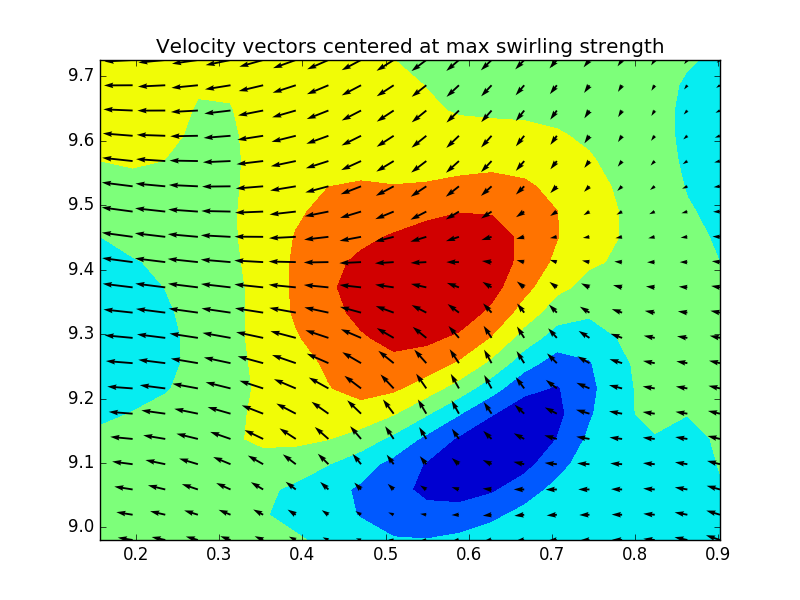
\includegraphics[scale=0.5]{figure/2.png}
	\caption{test}
\end{figure}

\begin{table}[h]
	\centering
	\caption{test table}
	\vspace{10px}
	\label{tb:test}
	\begin{tabular}{l|l|l|l|l}
		cores         & 1      & 2    & 4   & 8 [\%] \\
		\hline
		elapsed time  & 9.36  & 12.90  & 9.61 &  8.56 \\
		cpu time      & 9.36  & 25.81  & 38.55& 66.45 \\
		efficiency    & 1.00  & 0.73   & 0.97 & 1.09
	\end{tabular}
\end{table}

\newpage
\bibliographystyle{plain}
\bibliography{biblio}

\end{document}














